\documentclass{standalone}
\usepackage{tikz}
\usetikzlibrary{patterns, positioning}

\begin{document}
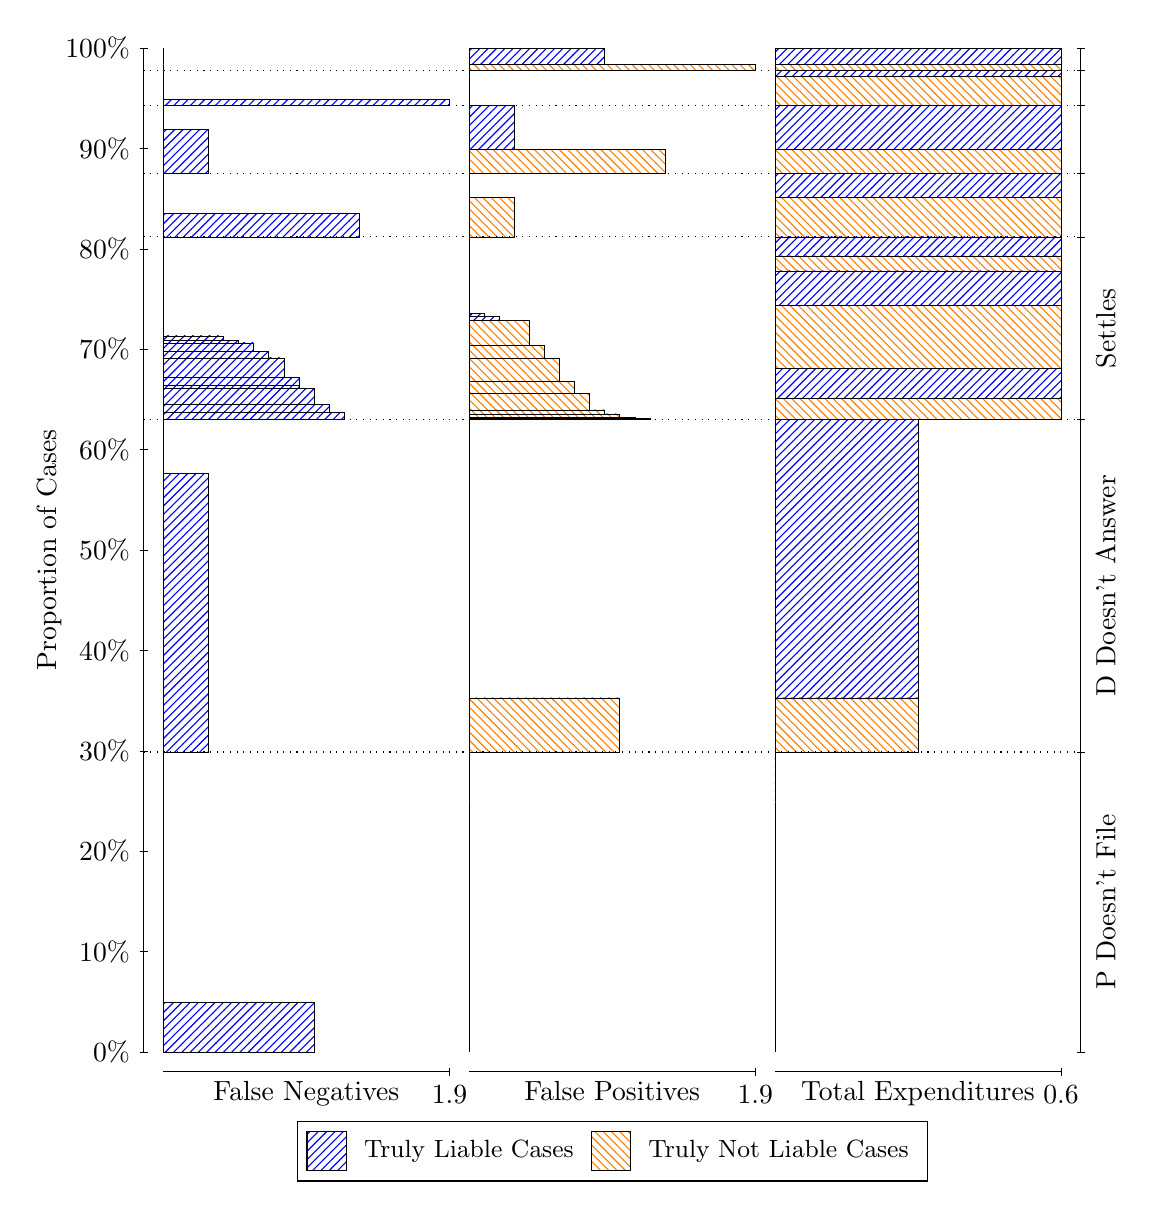
\begin{tikzpicture}
\draw[black, very thin] (1.5,1.75) -- (1.5,14.5);
\node[rotate=90, anchor=center] at (0.3, 8.125) {Proportion of Cases};
\draw[black, very thin] (1.45,1.75) -- (1.55,1.75);
\node[anchor=east] at (1.45, 1.75) {0\%};
\draw[black, very thin] (1.45,3.025) -- (1.55,3.025);
\node[anchor=east] at (1.45, 3.025) {10\%};
\draw[black, very thin] (1.45,4.3) -- (1.55,4.3);
\node[anchor=east] at (1.45, 4.3) {20\%};
\draw[black, very thin] (1.45,5.575) -- (1.55,5.575);
\node[anchor=east] at (1.45, 5.575) {30\%};
\draw[black, very thin] (1.45,6.85) -- (1.55,6.85);
\node[anchor=east] at (1.45, 6.85) {40\%};
\draw[black, very thin] (1.45,8.125) -- (1.55,8.125);
\node[anchor=east] at (1.45, 8.125) {50\%};
\draw[black, very thin] (1.45,9.4) -- (1.55,9.4);
\node[anchor=east] at (1.45, 9.4) {60\%};
\draw[black, very thin] (1.45,10.675) -- (1.55,10.675);
\node[anchor=east] at (1.45, 10.675) {70\%};
\draw[black, very thin] (1.45,11.95) -- (1.55,11.95);
\node[anchor=east] at (1.45, 11.95) {80\%};
\draw[black, very thin] (1.45,13.225) -- (1.55,13.225);
\node[anchor=east] at (1.45, 13.225) {90\%};
\draw[black, very thin] (1.45,14.5) -- (1.55,14.5);
\node[anchor=east] at (1.45, 14.5) {100\%};

\draw[black, very thin] (13.4,1.75) -- (13.4,14.5);
\draw[black, very thin] (13.35,1.75) -- (13.45,1.75);
\node[anchor=west] at (13.35, 1.75) {};
\draw[black, very thin] (13.35,5.5603) -- (13.45,5.5603);
\node[anchor=west] at (13.35, 5.5603) {};
\draw[black, very thin] (13.35,9.7802) -- (13.45,9.7802);
\node[anchor=west] at (13.35, 9.7802) {};
\draw[black, very thin] (13.35,12.101) -- (13.45,12.101);
\node[anchor=west] at (13.35, 12.101) {};
\draw[black, very thin] (13.35,12.908) -- (13.45,12.908);
\node[anchor=west] at (13.35, 12.908) {};
\draw[black, very thin] (13.35,13.772) -- (13.45,13.772);
\node[anchor=west] at (13.35, 13.772) {};
\draw[black, very thin] (13.35,14.215) -- (13.45,14.215);
\node[anchor=west] at (13.35, 14.215) {};
\draw[black, very thin] (13.35,14.5) -- (13.45,14.5);
\node[anchor=west] at (13.35, 14.5) {};

\draw[black, very thin, pattern color=blue, pattern=north east lines] (1.75,1.75) rectangle (3.6623,2.3795);
\draw[black, very thin, pattern color=orange, pattern=north west lines] (1.75,2.3795) rectangle (1.75,5.5603);
\draw[black, very thin, pattern color=blue, pattern=north east lines] (1.75,5.5603) rectangle (2.3237,9.0936);
\draw[black, very thin, pattern color=orange, pattern=north west lines] (1.75,9.0936) rectangle (1.75,9.7802);
\draw[black, very thin, pattern color=blue, pattern=north east lines] (1.75,9.7802) rectangle (4.0447,9.8732);
\draw[black, very thin, pattern color=blue, pattern=north east lines] (1.75,9.8732) rectangle (3.8535,9.972);
\draw[black, very thin, pattern color=blue, pattern=north east lines] (1.75,9.972) rectangle (3.6623,10.178);
\draw[black, very thin, pattern color=blue, pattern=north east lines] (1.75,10.178) rectangle (3.4711,10.216);
\draw[black, very thin, pattern color=blue, pattern=north east lines] (1.75,10.216) rectangle (3.4711,10.318);
\draw[black, very thin, pattern color=blue, pattern=north east lines] (1.75,10.318) rectangle (3.2798,10.564);
\draw[black, very thin, pattern color=blue, pattern=north east lines] (1.75,10.564) rectangle (3.0886,10.652);
\draw[black, very thin, pattern color=blue, pattern=north east lines] (1.75,10.652) rectangle (2.8974,10.754);
\draw[black, very thin, pattern color=blue, pattern=north east lines] (1.75,10.754) rectangle (2.7061,10.791);
\draw[black, very thin, pattern color=blue, pattern=north east lines] (1.75,10.791) rectangle (2.5149,10.843);
\draw[black, very thin, pattern color=orange, pattern=north west lines] (1.75,10.843) rectangle (1.75,12.101);
\draw[black, very thin, pattern color=blue, pattern=north east lines] (1.75,12.101) rectangle (4.236,12.404);
\draw[black, very thin, pattern color=orange, pattern=north west lines] (1.75,12.404) rectangle (1.75,12.908);
\draw[black, very thin, pattern color=blue, pattern=north east lines] (1.75,12.908) rectangle (2.3237,13.469);
\draw[black, very thin, pattern color=orange, pattern=north west lines] (1.75,13.469) rectangle (1.75,13.772);
\draw[black, very thin, pattern color=blue, pattern=north east lines] (1.75,13.772) rectangle (5.3833,13.85);
\draw[black, very thin, pattern color=orange, pattern=north west lines] (1.75,13.85) rectangle (1.75,14.215);
\draw[black, very thin, pattern color=orange, pattern=north west lines] (1.75,14.215) rectangle (1.75,14.292);
\draw[black, very thin, pattern color=blue, pattern=north east lines] (1.75,14.292) rectangle (1.75,14.5);
\draw[black, very thin, pattern color=orange, pattern=north west lines] (5.6333,1.75) rectangle (5.6333,4.9308);
\draw[black, very thin, pattern color=blue, pattern=north east lines] (5.6333,4.9308) rectangle (5.6333,5.5603);
\draw[black, very thin, pattern color=orange, pattern=north west lines] (5.6333,5.5603) rectangle (7.5456,6.2469);
\draw[black, very thin, pattern color=blue, pattern=north east lines] (5.6333,6.2469) rectangle (5.6333,9.7802);
\draw[black, very thin, pattern color=orange, pattern=north west lines] (5.6333,9.7802) rectangle (7.9281,9.7938);
\draw[black, very thin, pattern color=orange, pattern=north west lines] (5.6333,9.7938) rectangle (7.7368,9.8088);
\draw[black, very thin, pattern color=orange, pattern=north west lines] (5.6333,9.8088) rectangle (7.5456,9.8536);
\draw[black, very thin, pattern color=orange, pattern=north west lines] (5.6333,9.8536) rectangle (7.3544,9.9053);
\draw[black, very thin, pattern color=orange, pattern=north west lines] (5.6333,9.9053) rectangle (7.1632,10.115);
\draw[black, very thin, pattern color=orange, pattern=north west lines] (5.6333,10.115) rectangle (6.9719,10.27);
\draw[black, very thin, pattern color=orange, pattern=north west lines] (5.6333,10.27) rectangle (6.7807,10.559);
\draw[black, very thin, pattern color=orange, pattern=north west lines] (5.6333,10.559) rectangle (6.5895,10.721);
\draw[black, very thin, pattern color=orange, pattern=north west lines] (5.6333,10.721) rectangle (6.3982,11.039);
\draw[black, very thin, pattern color=blue, pattern=north east lines] (5.6333,11.039) rectangle (6.0158,11.091);
\draw[black, very thin, pattern color=blue, pattern=north east lines] (5.6333,11.091) rectangle (5.8246,11.127);
\draw[black, very thin, pattern color=blue, pattern=north east lines] (5.6333,11.127) rectangle (5.6333,12.101);
\draw[black, very thin, pattern color=orange, pattern=north west lines] (5.6333,12.101) rectangle (6.207,12.605);
\draw[black, very thin, pattern color=blue, pattern=north east lines] (5.6333,12.605) rectangle (5.6333,12.908);
\draw[black, very thin, pattern color=orange, pattern=north west lines] (5.6333,12.908) rectangle (8.1193,13.211);
\draw[black, very thin, pattern color=blue, pattern=north east lines] (5.6333,13.211) rectangle (6.207,13.772);
\draw[black, very thin, pattern color=orange, pattern=north west lines] (5.6333,13.772) rectangle (5.6333,14.137);
\draw[black, very thin, pattern color=blue, pattern=north east lines] (5.6333,14.137) rectangle (5.6333,14.215);
\draw[black, very thin, pattern color=orange, pattern=north west lines] (5.6333,14.215) rectangle (9.2667,14.292);
\draw[black, very thin, pattern color=blue, pattern=north east lines] (5.6333,14.292) rectangle (7.3544,14.5);
\draw[black, very thin, pattern color=orange, pattern=north west lines] (9.5167,1.75) rectangle (9.5167,4.9308);
\draw[black, very thin, pattern color=blue, pattern=north east lines] (9.5167,4.9308) rectangle (9.5167,5.5603);
\draw[black, very thin, pattern color=orange, pattern=north west lines] (9.5167,5.5603) rectangle (11.333,6.2469);
\draw[black, very thin, pattern color=blue, pattern=north east lines] (9.5167,6.2469) rectangle (11.333,9.7802);
\draw[black, very thin, pattern color=orange, pattern=north west lines] (9.5167,9.7802) rectangle (13.15,10.05);
\draw[black, very thin, pattern color=blue, pattern=north east lines] (9.5167,10.05) rectangle (13.15,10.434);
\draw[black, very thin, pattern color=orange, pattern=north west lines] (9.5167,10.434) rectangle (13.15,11.235);
\draw[black, very thin, pattern color=blue, pattern=north east lines] (9.5167,11.235) rectangle (13.15,11.671);
\draw[black, very thin, pattern color=orange, pattern=north west lines] (9.5167,11.671) rectangle (13.15,11.859);
\draw[black, very thin, pattern color=blue, pattern=north east lines] (9.5167,11.859) rectangle (13.15,12.101);
\draw[black, very thin, pattern color=orange, pattern=north west lines] (9.5167,12.101) rectangle (13.15,12.605);
\draw[black, very thin, pattern color=blue, pattern=north east lines] (9.5167,12.605) rectangle (13.15,12.908);
\draw[black, very thin, pattern color=orange, pattern=north west lines] (9.5167,12.908) rectangle (13.15,13.211);
\draw[black, very thin, pattern color=blue, pattern=north east lines] (9.5167,13.211) rectangle (13.15,13.772);
\draw[black, very thin, pattern color=orange, pattern=north west lines] (9.5167,13.772) rectangle (13.15,14.137);
\draw[black, very thin, pattern color=blue, pattern=north east lines] (9.5167,14.137) rectangle (13.15,14.215);
\draw[black, very thin, pattern color=orange, pattern=north west lines] (9.5167,14.215) rectangle (13.15,14.292);
\draw[black, very thin, pattern color=blue, pattern=north east lines] (9.5167,14.292) rectangle (13.15,14.5);
\draw[black, dotted] (1.5,5.5603) -- (13.4,5.5603);
\draw[black, dotted] (1.5,9.7802) -- (13.4,9.7802);
\draw[black, dotted] (1.5,12.101) -- (13.4,12.101);
\draw[black, dotted] (1.5,12.908) -- (13.4,12.908);
\draw[black, dotted] (1.5,13.772) -- (13.4,13.772);
\draw[black, dotted] (1.5,14.215) -- (13.4,14.215);
\draw[black, very thin] (1.75,1.5) -- (5.3833,1.5);
\node[anchor=north] at (3.5667, 1.5) {False Negatives};
\draw[black, very thin] (5.3833,1.45) -- (5.3833,1.55);
\node[anchor=north] at (5.3833, 1.45) {1.9};

\draw[black, very thin] (5.6333,1.5) -- (9.2667,1.5);
\node[anchor=north] at (7.45, 1.5) {False Positives};
\draw[black, very thin] (9.2667,1.45) -- (9.2667,1.55);
\node[anchor=north] at (9.2667, 1.45) {1.9};

\draw[black, very thin] (9.5167,1.5) -- (13.15,1.5);
\node[anchor=north] at (11.333, 1.5) {Total Expenditures};
\draw[black, very thin] (13.15,1.45) -- (13.15,1.55);
\node[anchor=north] at (13.15, 1.45) {0.6};

\node[black, centered, rotate=90] at (13.72, 3.6552) {P Doesn't File};
\node[black, centered, rotate=90] at (13.72, 7.6702) {D Doesn't Answer};
\node[black, centered, rotate=90] at (13.72, 10.941) {Settles};





\draw (7.449999999999999,1.5) node[draw=none] (baseCoordinate) {};
\begin{scope}[align=center]
        \matrix[scale=0.5, draw=black, below=0.5cm of baseCoordinate, nodes={draw}, column sep=0.1cm]{
            \node[rectangle, draw, minimum width=0.5cm, minimum height=0.5cm, pattern=north east lines, pattern color=blue] {}; &
            \node[draw=none, font=\small] (B) {Truly Liable Cases}; &
            \node[rectangle, draw, minimum width=0.5cm, minimum height=0.5cm, pattern=north west lines, pattern color=orange] {}; &
            \node[draw=none, font=\small] (B) {Truly Not Liable Cases}; \\
            };
\end{scope}

\end{tikzpicture}
\end{document}